\section{Prototype Zero}
After gathering information from user questionnaires, conducting a competitor analysis, and creating tasks and dialogues using the methods described earlier, we moved on to developing the first prototype of our application interface. We used a tool called Justinmind, which allowed us to build the prototype by defining various windows, their connections, and the overall look and feel of the application. This tool helped us create a simple, clear, but accurate representation of our idea and its functionalities.
In the rest of the chapter, we are going to illustrate the prototype, dividing it by its different functionalities. This walkthrough will show how each feature is designed to meet user needs and contribute to the overall user experience.
	\subsection{Login}
		The first section describes the login process required to access the application's features.
		\begin{figure}[htbp]
			\centering
			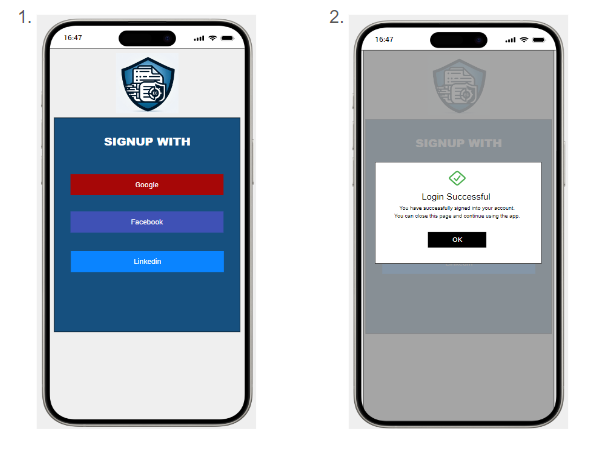
\includegraphics[width=0.80\textwidth]{../mockups/login.png}  % Replace 'example-image' with the filename of your image
		\end{figure}
		\clearpage
	\subsection{Add document from file system}
		The second section outlines the process of adding a document from saved files. It illustrates the steps you take, starting from opening the application to successfully adding a new document from a saved file.
		\begin{figure}[htbp]
			\centering
			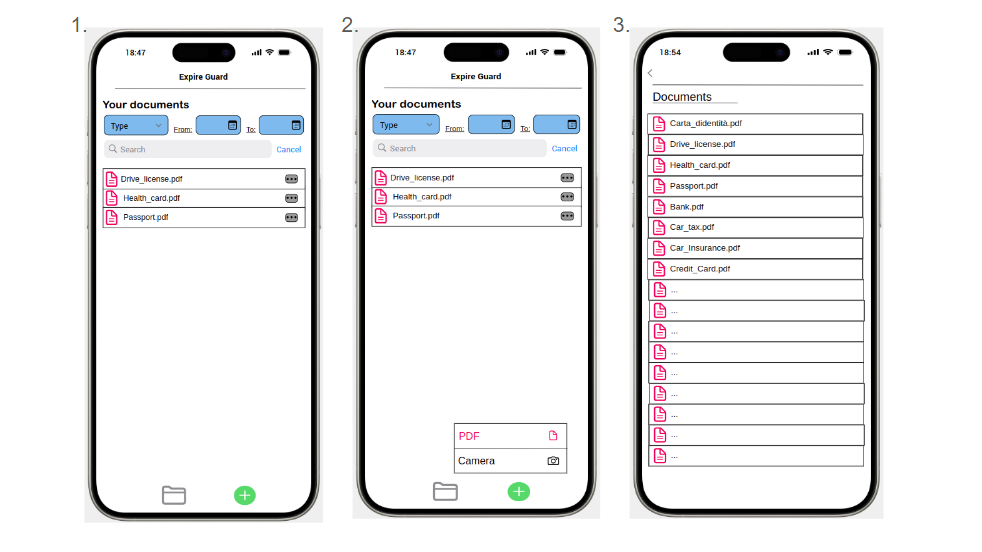
\includegraphics[width=0.80\textwidth]{../mockups/add_doc_pdf_1.png}  % Replace 'example-image' with the filename of your image
		\end{figure}
		
		\begin{figure}[htbp]
			\centering
			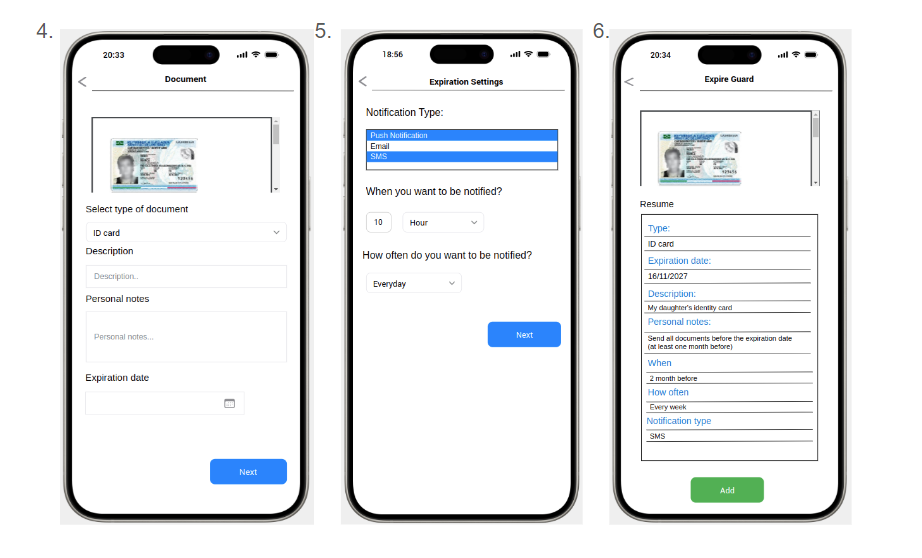
\includegraphics[width=0.75\textwidth]{../mockups/add_doc_pdf_2.png}  % Replace 'example-image' with the filename of your image
		\end{figure}
		\clearpage
	\subsection{Add document using camera scan}
		The third section is similar to the first one, but in this case, it illustrates the process of adding a document using the smartphone camera to scan it.
		\begin{figure}[htbp]
			\centering
			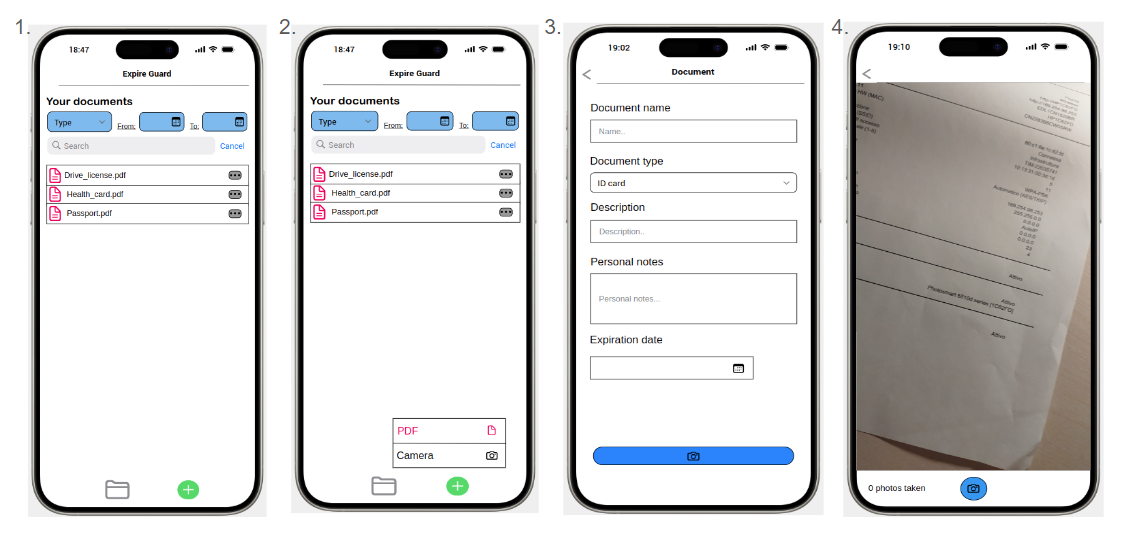
\includegraphics[width=0.9\textwidth]{../mockups/add_doc_cam_1.png}  % Replace 'example-image' with the filename of your image
		\end{figure}

		\begin{figure}[htbp]
			\centering
			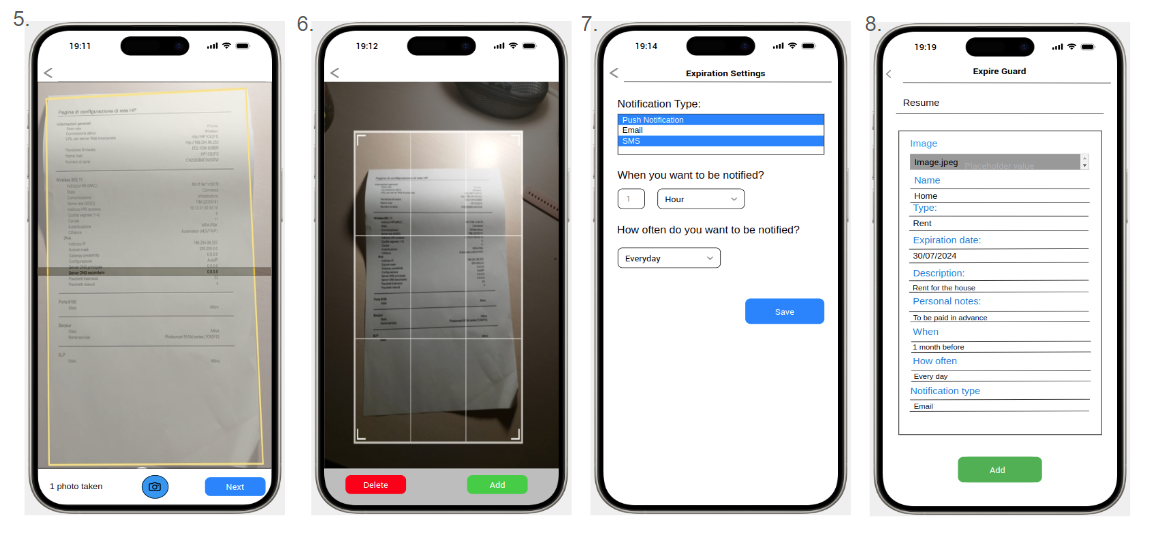
\includegraphics[width=0.9\textwidth]{../mockups/add_doc_cam_2.png}  % Replace 'example-image' with the filename of your image
		\end{figure}
		\clearpage
	\subsection{View document}
		The fourth section explains how to view the details of a saved document's. It also shows the presence of various filters on the document archive page to perform a custom search of saved documents.
		\begin{figure}[htbp]
			\centering
			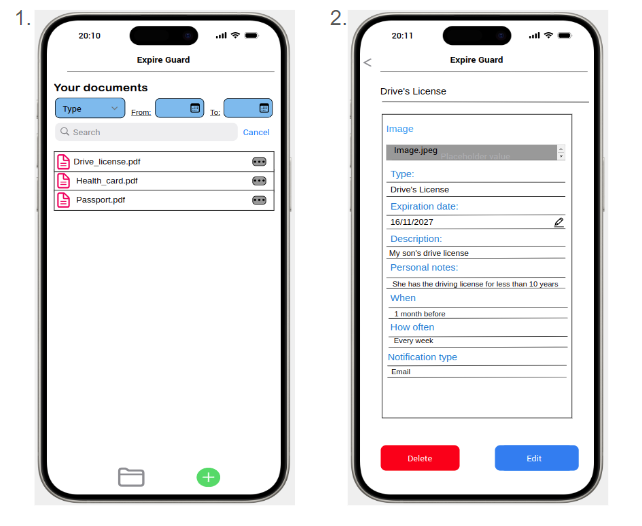
\includegraphics[width=0.7\textwidth]{../mockups/view_doc.png}  % Replace 'example-image' with the filename of your image
		\end{figure}
		\clearpage
	\subsection{Edit document description and personal notes}
		The fifth section illustrates the process of editing a saved document Description and Personal Notes.
		\begin{figure}[htbp]
			\centering
			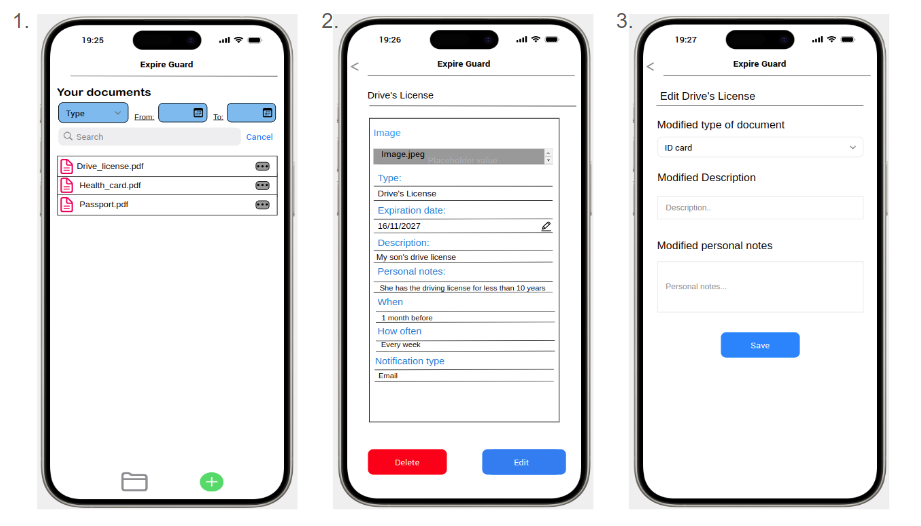
\includegraphics[width=0.9\textwidth]{../mockups/edit_doc_meta_1.png}  % Replace 'example-image' with the filename of your image
		\end{figure}
	
	\subsection{Edit document Expiration date and Expiration Settings}
		The sixth section illustrates the process of editing a saved document Expiration date and Expiration Settings.
		\begin{figure}[htbp]
			\centering
			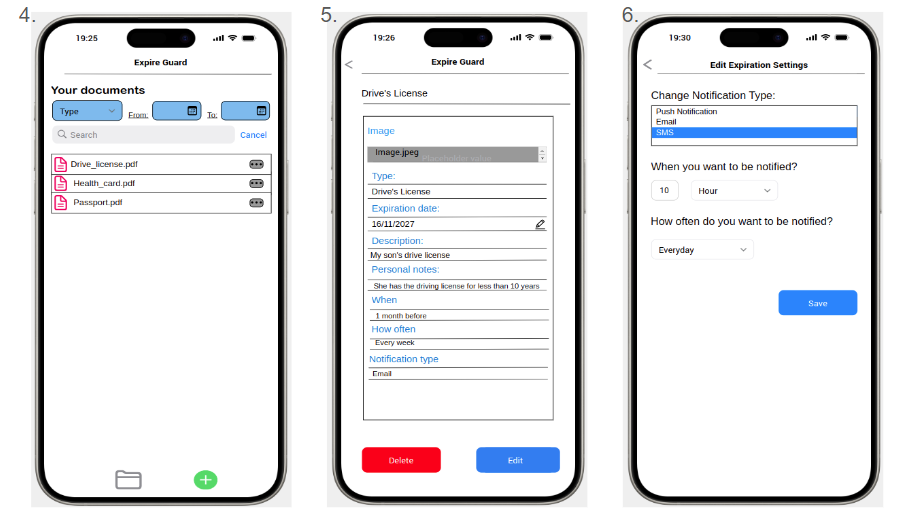
\includegraphics[width=0.9\textwidth]{../mockups/edit_doc_expr_1.png}  % Replace 'example-image' with the filename of your image
		\end{figure}
		\clearpage
	\subsection{Delete document}
		The last section illustrates the process of deleting a saved document.
		\begin{figure}[htbp]
			\centering
			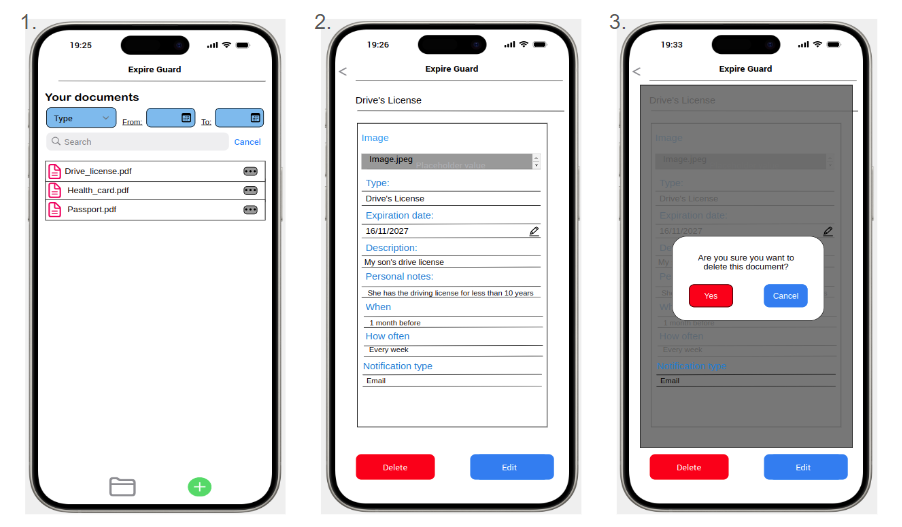
\includegraphics[width=0.9\textwidth]{../mockups/delete_doc.png}  % Replace 'example-image' with the filename of your image
		\end{figure}
		\clearpage
		
